\documentclass[aspectratio=43,english]{beamer} %If you want to create Polish presentation, replace 'english' with 'polish' and uncomment 3-th line, i.e., '\usepackage{polski}'
\usepackage[utf8]{inputenc}
\usepackage{polski} %Uncomment for Polish language
\usepackage{babel}
\usepackage{listings} %We want to put listings

\mode<beamer>{ 	%in 'beamer' mode
	\hypersetup{pdfpagemode=FullScreen}		%Enable Full screen mode
	\usetheme{JuanLesPins} 		%Show part title in right footer
	%\usetheme[dark]{AGH}                 		%Use dark background
	%\usetheme[dark,parttitle=leftfooter]{AGH}  	%Use dark background and show part title in left footer
}
\mode<handout>{	%in 'handout' mode
	\hypersetup{pdfpagemode=None}		
	\usepackage{pgfpages}
  	\pgfpagesuselayout{4 on 1}[a4paper,border shrink=5mm,landscape]	%show 4 slides on 1 page
  	\usetheme{boxes}
  	\addheadbox{structure}{\quad\insertpart\hfill\insertsection\hfill\insertsubsection\qquad} 	%content of header
 	\addfootbox{structure}{\quad\insertauthor\hfill\insertframenumber\hfill\insertsubtitle\qquad} 	%content of footer
}

\AtBeginPart{ %At begin part: display its name
	\frame{\partpage}
} 


%%%%%%%%%%% Configuration of the listings package %%%%%%%%%%%%%%%%%%%%%%%%%%
% Source: https://en.wikibooks.org/wiki/LaTeX/Source_Code_Listings#Using_the_listings_package
%%%%%%%%%%%%%%%%%%%%%%%%%%%%%%%%%%%%%%%%%%%%%%%%%%%%%%%%%%%%%%%%%%%%%%%%%%%%
\lstset{ %
  backgroundcolor=\color{white},   % choose the background color
  basicstyle=\footnotesize,        % the size of the fonts that are used for the code
  breakatwhitespace=false,         % sets if automatic breaks should only happen at whitespace
  breaklines=true,                 % sets automatic line breaking
  captionpos=b,                    % sets the caption-position to bottom
  commentstyle=\color{green},      % comment style
  deletekeywords={...},            % if you want to delete keywords from the given language
  escapeinside={\%*}{*)},          % if you want to add LaTeX within your code
  extendedchars=true,              % lets you use non-ASCII characters; for 8-bits encodings only, does not work with UTF-8
  frame=single,	                   % adds a frame around the code
  keepspaces=true,                 % keeps spaces in text, useful for keeping indentation of code (possibly needs columns=flexible)
  keywordstyle=\color{blue},       % keyword style
  morekeywords={*,...},            % if you want to add more keywords to the set
  numbers=left,                    % where to put the line-numbers; possible values are (none, left, right)
  numbersep=5pt,                   % how far the line-numbers are from the code
  numberstyle=\tiny\color{gray},   % the style that is used for the line-numbers
  rulecolor=\color{black},         % if not set, the frame-color may be changed on line-breaks within not-black text (e.g. comments (green here))
  showspaces=false,                % show spaces everywhere adding particular underscores; it overrides 'showstringspaces'
  showstringspaces=false,          % underline spaces within strings only
  showtabs=false,                  % show tabs within strings adding particular underscores
  stepnumber=2,                    % the step between two line-numbers. If it's 1, each line will be numbered
  stringstyle=\color{cyan},        % string literal style
  tabsize=2,	                   % sets default tabsize to 2 spaces
  title=\lstname,                  % show the filename of files included with \lstinputlisting; also try caption instead of title
                                   % needed if you want to use UTF-8 Polish chars
  literate={?}{{\k{a}}}1
           {?}{{\k{A}}}1
           {?}{{\k{e}}}1
           {?}{{\k{E}}}1
           {�}{{\'o}}1
           {�}{{\'O}}1
           {?}{{\'s}}1
           {?}{{\'S}}1
           {?}{{\l{}}}1
           {?}{{\L{}}}1
           {?}{{\.z}}1
           {?}{{\.Z}}1
           {?}{{\'z}}1
           {?}{{\'Z}}1
           {?}{{\'c}}1
           {?}{{\'C}}1
           {?}{{\'n}}1
           {?}{{\'N}}1
}
%%%%%%%%%%%%%%%%%


\title{Metody Obliczeniowe w Nauce i Technice}
\author{Marian Bubak, PhD}
\date{}
\institute[AGH]{
	Institute of Computer Science\\ul. Kawiory 21\\30-055 Krakow\\
	Poland\\
	\url{http://www.icsr.agh.edu.pl/~mownit/}
}



\subtitle{2. Arytmetyka komputerowa}
\begin{document}
  	\maketitle
	%%%%%%%%%%%%%%%%
	\begin{frame}{Outline}
		\tableofcontents
	\end{frame}
	%%%%%%%%%%%%%%%%
	\section{Numeryczna reprezentacja liczb całkowitych}
	%%%%%%%%%%%%%%%%
	\begin{frame}{Reprezentacja stałopozycyjna (integer)}
		np. kod U2: na d+1 bitach reprezentowane dokładnie liczby
        \[
        L \in [-2^d, 2^d-1]
        \]
        gdy argumenty, wynik reprezentowane stałopozycyjnie, to działania na nich: $+$, $-$, $\cdot$, $/ (div)$, $/ (mod)$ są wykonywane dokładnie
	\end{frame}
	%%%%%%%%%%%%%%%%
	\section{Numeryczna reprezentacja liczb rzeczywistych}
	%%%%%%%%%%%%%%%%
	\begin{frame}{Reprezentacja zmiennoprzecinkowa (float)}
    	Należy pamiętać o ułomności reprezentacji zbioru liczb rzeczywistych $\mathbb{R}$ w rzeczywistym świecie skończonych komputerów.
        \begin{block}{}
        $F$ - zbiór liczb zmiennoprzecinkowych (floating-point):\newline
        \begin{columns}
        	\column{0.45\linewidth}
                $\beta$ - podstawa,\newline
                $t$ - dokładność,\newline
                $L, U$ - zakres wykładnika\newline
            \column{0.45\linewidth}
            	$d_i$ - liczby całkowite,
                $0 \le d_i \le \beta - 1, i=1,...,t$
                $L \le e \le U$
        \end{columns}
        $x \in F$ ma wartość:
        \[
        x = \pm \underbrace{\left(\frac{d_1}{\beta} + \frac{d_2}{\beta^2} + ... + \frac{d_t}{\beta^t}\right)}_\text{mantysa} \cdot \beta^{\overbrace{e}^\text{cecha}}
        = \pm \sum_{i/1}^{t} \frac{d_i}{\beta^i} \cdot \beta^e
        \]        
		System $F$ jest {\it unormowany}, gdy $\forall_{x \ne 0} d_i \ne 0$.
        \end{block}
        
	\end{frame}
	%%%%%%%%%%%%%%%%
	\begin{frame}{Reprezentacja zmiennoprzecinkowa (float)}
        W komputerze jest przechowywana liczba całkowita $\beta^t \cdot m$ (zgodnie z wybranym systemem kodowania).
        
        $\beta^{1-t}$ - oszacowanie względnej dokładności arytmetyki
        
        \hspace{0.5cm}
        \centering
        \begin{tabular}{| l | c | c | c | c | c |}
        \hline
        Komputer & $\beta$ & $t$ & $L$ & $U$ & $\beta^{1-t}$ \\ \hline
        CDC CYBER 72 		& 2  & 48 & -975 	& 1070 & $7.11 \cdot 10^{-15}$ \\ \hline
        Cray-1 				& 2  & 48 & -16384	& 8191 & $7.11 \cdot 10^{-15}$ \\ \hline
        IBM 360, 370 		& 16 & 6  & -64		& 63   & $9.54 \cdot 10^{-7}$ \\ \hline
        IBM 360, 370 (DP) 	& 16 & 14 & -64 	& 63   & $2.22 \cdot 10^{-16}$ \\ \hline
        IBM PC XT / AT 		& & & & & \\ \hline
        Delta (VAX) 		& & & & & \\ \hline
        \end{tabular}
 	\end{frame}
	%%%%%%%%%%%%%%%%
	\begin{frame}{Reprezentacja zmiennoprzecinkowa (float)}
    	\begin{block}{Ważne}
        $F$ nie jest kontinuum - więcej - jest skończony o liczbie elementów wyrażonych wzorem:
        \[
        2 \cdot \left(\beta - 1 \right) \cdot \beta^{t-1} \cdot \left( U - L + 1 \right) + 1
        \]
        \begin{flushright}
        	{\it Zadanie:} sprawdzić
        \end{flushright}
        \end{block}
 	\end{frame}
	%%%%%%%%%%%%%%%%
	\begin{frame}{Reprezentacja zmiennoprzecinkowa (float)}
    	Elementy $F$ nie są równomiernie rozłożone na osi:
        $\beta = 2, t = 3, L = -1, U = 2$ \hspace{5mm} (33 elementy):
        \begin{center}
        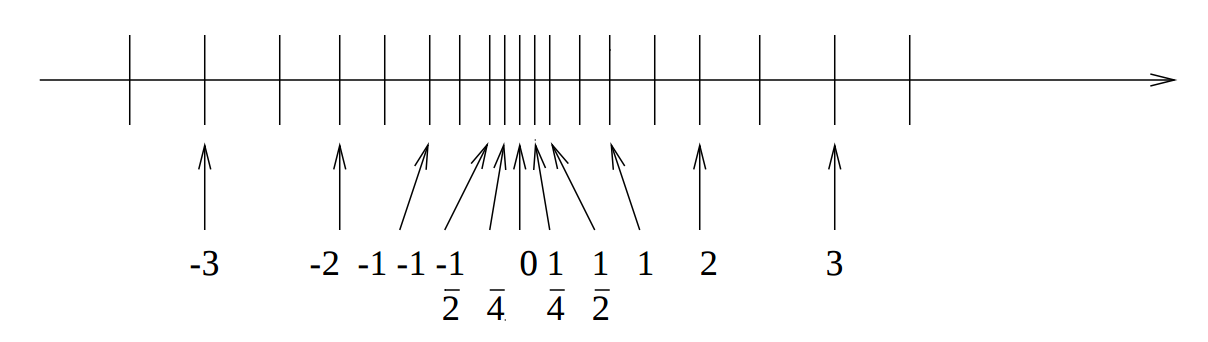
\includegraphics[width=0.8\linewidth]{img/2/2_1_axis}
        \end{center}
        
       	Każdy element $F$ reprezentuje cały przedział liczb $\mathbb{R}$\newline 
       	$x$ - l. rzeczywista $\in$ zakresu $F$,\newline
        $fl(x)$ - reprezentacja zmiennoprzecinkowa liczby $x$
        
        \[
        \left| \frac{fl(x) - x}{x} \right| \le \frac{1}{2} \beta^{1-t}
        \]
        
        \begin{flushright}
        	{\it Zadanie:} sprawdzić
        \end{flushright}
 	\end{frame}
	%%%%%%%%%%%%%%%%
	\begin{frame}{Reprezentacja zmiennoprzecinkowa (float)}
    	\begin{alertblock}{Uwaga}
    		$0.1$ - często krok w algorytmach\newline
            Czy 10 kroków o długości $0.1$ to to samo co 1 krok = $1.0$?\newline
            W systemie o $\beta = 2^n$ - {\bf nie!}
            \[
            0.1_{10} = 0.0(0011)_2 = 0.0(12)_4 = 0.0(6314)_8 = 0.199999..._{16}
            \]
            
            Reprezentacja $0.1$ urywa się o $t$ cyfrach. Dodanie 10 tak uzyskanych liczb nie da dokładnie $1.0$.
    	\end{alertblock}
 	\end{frame}
	%%%%%%%%%%%%%%%%
    \subsection{Dokładność reprezentacji zmiennoprzecinkowej}
	\begin{frame}{Reprezentacja zmiennoprzecinkowa (float)}
    	\[
        x = s \cdot 2^c \cdot m
        \]\[
        m = \sum_{i/1}^{\infty} e_i \cdot 2^{-i}
        \]\[
        e_i = \left\{ 
                  \begin{array}{ll}
                      0 \\
                      1
                  \end{array}
            \right.
        \]
        
        \begin{block}{Reprezentacja mantysy}
            Mantysa jest reprezentowana jako:
            \[
            m_t = \sum_{i/1}^{t}e_i \cdot 2^{-i} + \underbrace{e_{t+1} \cdot 2^{-t}}_\text{zaokrąglenie}
            \]
        \end{block}
 	\end{frame}
	%%%%%%%%%%%%%%%%
	\begin{frame}{Reprezentacja zmiennoprzecinkowa (float)}
    	a)\newline
        
    	\centering
        \begin{tabular}{|*{5}{p{.75cm}|}}
        	\hline
            t & t+1 & t+2 & ... &  \\ \hline
              & 0   & 1   & ... & 1 \\ \hline
        \end{tabular}
        \[
        m = \underbrace{\sum_{i/1}^{t} e_i \cdot 2^{-i} + 0 \cdot 2^{-(t+1)}}_{m_t} +
        	\underbrace{\sum_{i/t+2}^{\infty} 1 \cdot 2^{-i}}_{
            	\frac{1}{2^{t+1}} = 2^{-(t+1)}
            }
        \] \[
        m - m_t = 2^{-(t+1)}
        \]
 	\end{frame}
	%%%%%%%%%%%%%%%%
	\begin{frame}{Reprezentacja zmiennoprzecinkowa (float)}
    	b)\newline
        
    	\centering
        \begin{tabular}{|*{5}{p{.75cm}|}}
        	\hline
            t & t+1 & t+2 & ... &  \\ \hline
              & 1   & 0   & ... & 0 \\ \hline
        \end{tabular}
        \[
        m = \sum_{i/1}^{t} e_i \cdot 2^{-i} + 2^{-(t+1)}
        \]\[
        m_t = \sum_{i/1}^{t} e_i \cdot 2^{-i} + 2^{-t}
        \] \[
        m_t - m = 2^{-(t+1)} \left| \frac{m - m_t}{m} \right| \le \frac{2^{-(t+1)}}{1/2} = 2^{-t}
        \]
 	\end{frame}
	
	%%%%%%%%%%%%%%%%
    \section{Operacje zmiennopozycyjne}
    %%%%%%%%%%%%%%%%
    \begin{frame}{Operacje zmiennopozycyjne}
    	$x, y \in F$ \newline
        $x + y \in^? F$
        
        \begin{center}
        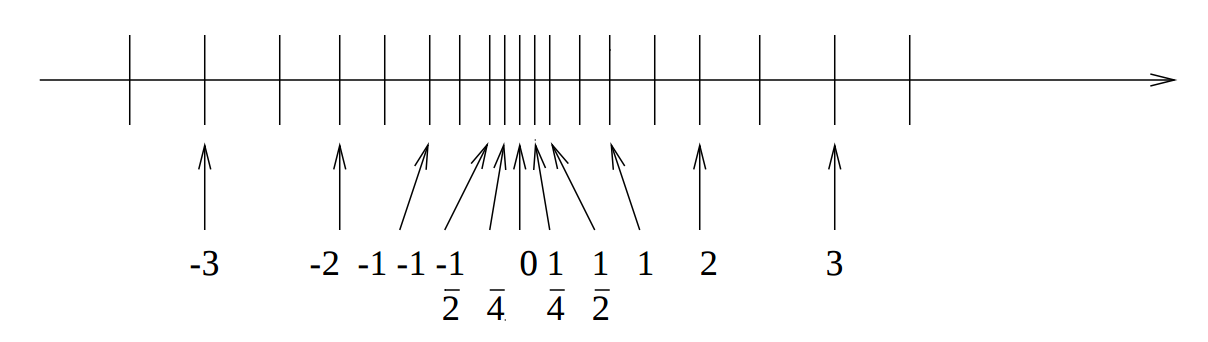
\includegraphics[width=0.8\linewidth]{img/2/2_1_axis}
        \end{center}
        System z powyższego rysunku: $\frac{5}{4} + \frac{3}{8} \notin F$ - ze względu na ,,gęstość'' elementów $F$.
    \end{frame}
    %%%%%%%%%%%%%%%%
    \begin{frame}{Operacje zmiennopozycyjne}
        $\frac{7}{2} + \frac{7}{2} \notin F$ - {\it overflow}
        \vspace{.5cm}
        
        W większości komputerów: $x \oplus y = fl(x + y)$ dla $x + y$ z zakresu $F$
        
        $\oplus$ - dodawanie zmiennopozycyjne, \newline
        $fl$ - reprezentacja
        
        \[
        a + b = 2^{c_a} \cdot \left( m_a + m_b \cdot 2^{-(c_a-c_b)} \right) \Rightarrow
        \left\{ 
            \begin{array}{ll}
                |b| \le 1/2 \cdot 2^{-t} \cdot |a| \\
                fl(a + b) = a
            \end{array}
        \right.
        \]
    \end{frame}
    %%%%%%%%%%%%%%%%
    \begin{frame}{Operacje zmiennopozycyjne}
    	$x + y$ rzadko $\in F$, bo:
        \begin{itemize}
        \item $x \cdot y$ ma $2 \cdot t$ lub $2 \cdot t - 1$ cyfr znaczących,
        \item {\it overflow} - bardziej prawdopodobny
        \item {\it underflow} - bardziej prawdopodobny
        \item $\oplus, \odot$
        	\begin{itemize}
            \item są {\it przemienne}
            \item nie są {\it łączne}, {\it rozdzielne}
            \end{itemize}
        \end{itemize}
    \end{frame}
    %%%%%%%%%%%%%%%%
    \begin{frame}{Operacje zmiennopozycyjne}
    	Ogólnie:
    	\[
        fl(a \square b) = rd(a \square b) = (a \square b) \cdot (1 + \varepsilon)
    	\] \[
        \varepsilon = \varepsilon(a, b, \square), \varepsilon \le \beta^{1-t}
        \] \[
        \square = +, -, \cdot, /
        \]
        
        \begin{block}{Definicja}
            {\bf Maszynowe $\varepsilon$} - najmniejsza liczba zmiennoprzecinkowa, dla której jeszcze: \[
            1 \oplus \varepsilon > 1
            \]
        \end{block}
        
        Zwykle wystarcza znajomość $\varepsilon' = 2^k \cdot \varepsilon, k \approx 1, 2, 3, ...$ $\rightarrow$ fragment progr. $\varepsilon$
    \end{frame}
\end{document}
